% ASPECT-D — DiffuLM @ NeurIPS 2026 extended abstract (4 pages main text)
% Phase 7 populates every [TODO:...] from artifacts/fits.json + artifacts/runs.csv
% following paper/OUTLINE.md. Do not add claims outside the declared outcome class.
\documentclass{article}

% TODO(style): download neurips_2026.sty from the NeurIPS 2026 Call for Papers page
% and use \usepackage{neurips_2026}. If the file cannot be fetched in this
% environment, leave this TODO in place and note it in DECISION.md — do NOT
% silently substitute another year's style file.
% \usepackage{neurips_2026}

\usepackage[utf8]{inputenc}
\usepackage[T1]{fontenc}
\usepackage{amsmath,amssymb}
\usepackage{booktabs}
\usepackage{graphicx}
\usepackage{xcolor}

\title{[TODO: title per OUTLINE.md, matched to declared outcome class]}
\author{Anonymous authors\\Paper under double-blind review}

\begin{document}
\maketitle

\begin{abstract}
[TODO: 120--150 words. Sentence 1: diffusion LMs decouple owned serial compute
(depth) from rented serial compute (denoising steps). Sentence 2: design — iso-N
width--depth grid $\times$ inference-time step sweep for zero-shot TTS, per-metric
laws. Sentences 3--4: headline numbers — $\Delta\tau$ CI, $\kappa_{\mathrm{WER}}$
CI, outcome class in plain words. Sentence 5: serving implication.]
\end{abstract}

\section{Introduction}
[TODO per OUTLINE.md \S1. Key display equation early:]
\begin{equation}
\mathrm{err}_m(w,d,T) \;=\; E_m + A_m w^{-\alpha_m} + B_m d^{-\beta_m} + C_m T^{-\tau_m}
\qquad
\mathrm{err}_m \;=\; E_m + A_m w^{-\alpha_m} + B_m \big(d\,T^{\kappa_m}\big)^{-\beta_m}
\end{equation}

\section{Related work}
[TODO per OUTLINE.md \S2.]

\section{Method}
[TODO per OUTLINE.md \S3. Must state: run-level bootstrap; frozen sampler
(MaskGIT confidence decode, $T$ steps per codebook level, NFE $=8T$, no CFG);
matched per-item RNG across $T$; $\mu$P + depth-transfer gate.]

\section{Results}
% Fig 1
\begin{figure}[t]
  \centering
  % 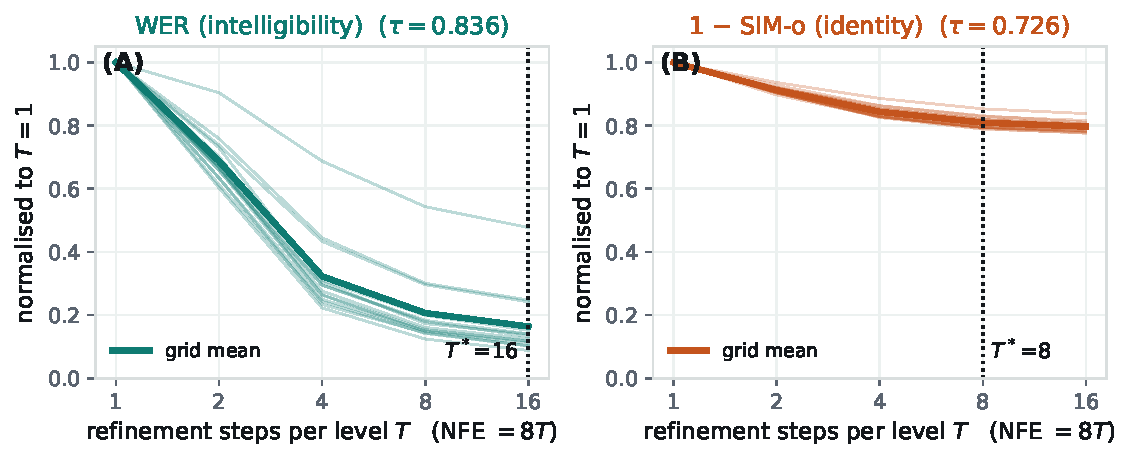
\includegraphics[width=.48\linewidth]{../artifacts/figures/step_curves.pdf}
  % 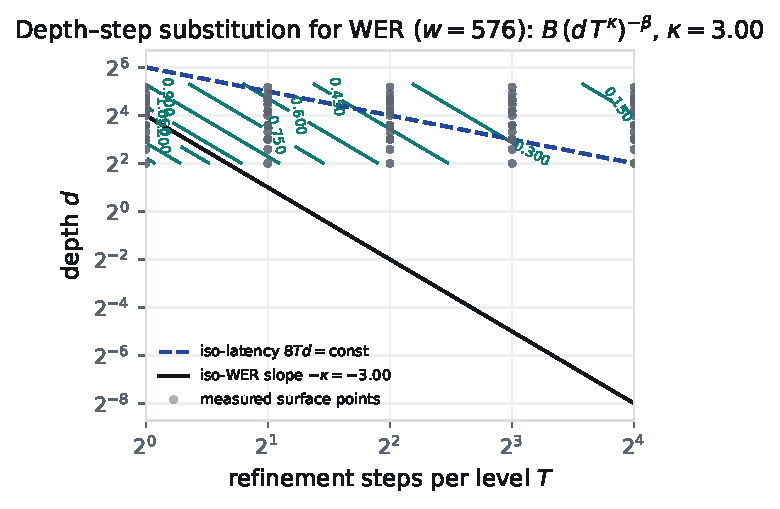
\includegraphics[width=.48\linewidth]{../artifacts/figures/substitution_plane.pdf}
  \caption{[TODO: (left) error vs.\ $T$ per metric, normalized, saturation steps
  $T^{*}_m$ marked; (right) fitted iso-WER contours in $(\log T, \log d)$ with
  slope $-\kappa_{\mathrm{WER}}$ and the iso-latency line $8Td=\text{const}$.]}
  \label{fig:main}
\end{figure}

% Table 1 — never cut this table (OUTLINE.md hard rules)
\begin{table}[t]
  \centering
  \caption{[TODO: fitted exponents per metric with 95\% CIs; $\Delta\tau$ bolded;
  AICc for $M_{\mathrm{sep}}$ / $M_{\mathrm{sub}}$ / $N$-only.]}
  \begin{tabular}{lcccccc}
    \toprule
    Metric & $\alpha$ (width) & $\beta$ (depth) & $\tau$ (steps) & $\kappa$ &
    $\Delta$AICc$_{\mathrm{sub-sep}}$ & $\Delta$AICc$_{\mathrm{full}-N}$\\
    \midrule
    WER   & [TODO] & [TODO] & [TODO] & [TODO] & [TODO] & [TODO]\\
    SIM-o & [TODO] & [TODO] & [TODO] & [TODO] & [TODO] & [TODO]\\
    \bottomrule
  \end{tabular}
  \label{tab:exponents}
\end{table}

[TODO per OUTLINE.md \S4: H-D2 and H-D3 with CIs first; then H-D1 at $T{=}16$;
H-D4 extrapolation; DegenRate($T$); serving corollary + populated latency table
with measured $c_{\mathrm{layer}}$.]

\section{Limitations and outlook}
[TODO per OUTLINE.md \S5, including any calendar cuts taken, stated exactly.]

\paragraph{Reproducibility.}
[TODO: pre-registered protocol, frozen sampler, released runs and fits;
anonymized artifact placeholder during review.]

% \bibliographystyle{plainnat}
% \bibliography{refs}
\end{document}
